\documentclass[11pt]{article}
\usepackage[scaled=0.92]{helvet}
\usepackage{geometry}
\geometry{letterpaper,tmargin=1in,bmargin=1in,lmargin=1in,rmargin=1in}
\usepackage[parfill]{parskip} % Activate to begin paragraphs with an empty line rather than an indent %\usepackage{graphicx}
\usepackage{amsmath,amssymb, mathrsfs,  mathtools, dsfont}
\usepackage{tabularx}
\usepackage{tikz-cd}
\usepackage[font=footnotesize,labelfont=bf]{caption}
\usepackage{graphicx}
\usepackage{xcolor}
%\usepackage[linkbordercolor ={1 1 1} ]{hyperref}
%\usepackage[sf]{titlesec}
\usepackage{natbib}
\usepackage{../../Tianpei_Report}

%\usepackage{appendix}
%\usepackage{algorithm}
%\usepackage{algorithmic}

%\renewcommand{\algorithmicrequire}{\textbf{Input:}}
%\renewcommand{\algorithmicensure}{\textbf{Output:}}



\begin{document}
\title{Lecture 11: The Cotangent Bundle}
\author{ Tianpei Xie}
\date{Oct. 16th., 2022}
\maketitle
\tableofcontents
\newpage
\section{Covectors}
\subsection{Covectors on Vector Space}
\begin{itemize}
\item \emph{Tangent covectors} are \emph{linear functionals} on the tangent space at a point $p \in M$.  The space of all covectors at $p$ is a vector space called the \emph{cotangent space} at $p$; in linear-algebraic terms, it is the \emph{dual space} to tangent space $T_{p}M$. \citep{lee2003introduction}

\item Whereas \emph{tangent vectors} give us a \emph{coordinate-free} interpretation of derivatives of curves, it turns out that derivatives of \emph{real-valued functions} on a manifold are most naturally interpreted as \emph{tangent covectors}.

\item \begin{definition}
Let $V$ be a \emph{finite-dimensional real vector space}. We define a \underline{\emph{\textbf{covector}}} on $V$ to be a \textbf{\emph{real-valued linear functional}} on $V$, that is, a \emph{linear map} $\omega: V \rightarrow \bR$.

\emph{\textbf{The space of all covectors}} on $V$ is itself a \emph{real vector space} under the obvious operations of \emph{pointwise addition} and \emph{scalar multiplication}. It is denoted by $V^{*}$ and called the \underline{\emph{\textbf{dual space}}} of $V$.
\end{definition}

\item Note that $V$ can be a space of vector space of functionals itself. And a functional of functionals is a functional, since a \emph{functional} is a function of functions.

\item \begin{proposition}
Let $V$ be a finite-dimensional vector space. Given any basis $(E_1,\ldots, E_n)$ for $V$, let $\epsilon^1, \ldots, \epsilon^n \in V^{*}$ be the covectors defined by 
\begin{align*}
\epsilon^{i}(E_{j}) &= \delta_{j}^{i}
\end{align*}
where $\delta_{j}^{i}$ is the Kronecker delta symbol. Then $\epsilon^1, \ldots, \epsilon^n$ is a \textbf{basis} for $V^{*}$, called the \textbf{dual basis} to $(E_j)$. Therefore, $\text{dim}\,V^{*} = \text{dim}\,V$.
\end{proposition}

\item \begin{example}
For example, we can apply this to \emph{\textbf{the standard basis}} $(e_1, \ldots, e_n)$ for $\bR^n$. The \emph{dual basis} is denoted by $(e^1,\ldots,e^n)$ (note the \emph{upper indices}), and is called \emph{\textbf{the standard dual basis}}. These basis \emph{covectors} are the \emph{linear functionals} on $\bR^n$ given by
\begin{align}
e^{i}(v) &= e^{i}(v^1,\ldots, v^{n}) = v^{i}. \label{eqn: covector_basis_vector_basis}
\end{align} In other words, $e^i$ is the linear functional that \emph{picks out the $i$-th component of a vector}. 

In \textbf{matrix notation}, a linear map from $\bR^n$ to $\bR$ is represented by a $1 \times n$ matrix, called a \emph{\textbf{row matrix}}. The \emph{\textbf{basis covectors}} can therefore also be thought of as the linear functionals represented by the \emph{row matrices}
\begin{align}
e^{i} = (0,\ldots, 1, \ldots, 0), \quad i=1,\ldots, n \label{eqn: covector_basis_row_mat}
\end{align} where $i$-th element is $1$ and the others are all zeros.
\end{example}

\item In general, if $(E_j)$ is a basis for $V$ and $(\epsilon^i)$ is its dual basis, then for any vector
$v = v^j E_j \in V$, we have (using the summation convention)
\begin{align*}
\epsilon^{i}(v) &= \epsilon^{i}(v^j E_j) = v^j \epsilon^{i}(E_j) = v^j \delta_{j}^{i} = v^{i}
\end{align*} Thus,just as in the case of $\bR^n$, the $i$-th basis covector $\epsilon^i$ picks out the $i$-th component of a vector with respect to the basis $(E_j)$.

\item  More generally, we can express an arbitrary covector $\omega \in V^{*}$ in terms of the \emph{dual basis} as
\begin{align}
\omega & = \omega_i \epsilon^{i} \label{eqn: covector_linear_reprsent_via_basis}
\end{align} where the components are determined by $\omega_i = \omega(E_i)$. 

The \emph{\textbf{action}} of $\omega$ on a vector $v = v^j E_j$ is
\begin{align}
\omega(v) &= \omega_i \epsilon^{i}(v) = \omega_i\, v^{i} \label{eqn: covector_act_on_vector}
\end{align}

\item Note that we always write \emph{\textbf{basis covectors}} \emph{with \textbf{upper indices}}, and \emph{\textbf{components}} of a covector \emph{with \textbf{lower indices}}, because this helps to ensure that mathematically meaningful summations such as \eqref{eqn: covector_linear_reprsent_via_basis} and \eqref{eqn: covector_act_on_vector} always follow our index conventions.

\item 
\begin{definition}
Suppose $V$ and $W$ are vector spaces and $A: V \rightarrow W$ is a \emph{linear map}. We define a linear map $A^{*}: W^{*} \rightarrow V^{*}$, called \underline{\emph{\textbf{the dual map}}} or \textbf{\emph{transpose of $A$}}, by
\begin{align}
(A^{*}\,\omega)(v) &= \omega\paren{A\,v}, \quad \forall\, \omega \in W^{*}, \; v \in V. \label{eqn: dual_map}
\end{align}
\end{definition}

\item 
\begin{proposition}
The \textbf{dual map} satisfies the following properties:
\begin{enumerate}
\item  $(A \circ B)^{*} = B^{*} \circ A^{*}$.
\item  $(\text{Id}_{V})^{*}: V^{*} \rightarrow V^{*}$ is the identity map of $V^{*}$.
\end{enumerate}
\end{proposition}

\item \begin{corollary}
The assignment that sends a vector space to its dual space and a linear map to its dual map is a \textbf{contravariant functor} from the category of real vector spaces to itself.
\end{corollary}

\item \begin{definition}
Apart from the fact that the dimension of $V^{*}$ is the same as that of $V$, the second most important fact about dual spaces is the following characterization of the \emph{\textbf{second dual space}} $V^{**} = (V^{*})^{*}$.

For each vector space $V$ there is a natural, \emph{\textbf{basis-independent map}} $\xi: V \rightarrow V^{**}$, defined as follows. For each vector $v \in V$, define a \emph{\textbf{linear functional}} $\xi(v): V^{*} \rightarrow \bR$ by
\begin{align}
\xi(v)(\omega) = \omega(v), \quad \forall \omega \in V^{*}. \label{eqn: double_dual_vector}
\end{align}
\end{definition}

\item \begin{proposition}
For any finite-dimensional vector space $V$, the map $\xi: V \rightarrow V^{**}$ is an \textbf{isomorphism}.
\end{proposition}

\item \begin{remark} Some of important things to note:
\begin{itemize}
\item The preceding proposition shows that when $V$ is finite-dimensional, we can unambiguously \textbf{\emph{identify}} $V^{**}$ with $V$ itself, because the map $\xi$ is \emph{canonically defined}, without reference to any basis. 

\item It is important to observe that although $V^{*}$ is \emph{also \textbf{isomorphic}} to $V$ (for the simple reason that any two finite-dimensional vector spaces of the same dimension are isomorphic), there is \emph{\textbf{no canonical isomorphism}} $V \simeq V^{*}$.

\item Because of Proposition above, the real number $\omega(v)$ obtained by applying a covector $\omega$ to a vector $v$ is sometimes denoted by either of the more \emph{\textbf{symmetric-looking notations}} $\inn{\omega}{v}$ and $\inn{v}{\omega}$, both expressions can be thought of either as \emph{\textbf{the action of the covector $\omega \in V^{*}$ on the vector $v \in V$}}, or as \emph{\textbf{the action of the linear functional $\xi(v) \in V^{**}$ on the element $\omega \in V^{*}$}}. 

There should be no cause for confusion with the use of the same angle bracket notation for inner products: \emph{whenever one of the arguments is a \textbf{vector} and the other a \textbf{covector}}, the notation $\inn{\omega}{v}$ is always to be interpreted as the \emph{\textbf{natural pairing}} between vectors and covectors, \emph{not as an inner product}. We typically omit any mention of the map $\xi$, and think of $v \in V$ \emph{either as a \textbf{vector}} or as \emph{a \textbf{linear functional}} on $V^{*}$, depending on the context.

\item There is also a \textbf{\emph{symmetry}} between \emph{\textbf{bases}} and \emph{\textbf{dual bases}} for a finite-dimensional vector space $V$: any \emph{basis} for $V$ determines a \emph{dual basis} for $V^{*}$, and \emph{\textbf{conversely}}, any \emph{basis} for $V^{*}$ determines a \emph{dual basis} for $V^{**} = V$. 

If $(\epsilon^i)$ is the basis for $V^{*}$ \emph{dual} to a basis $(E_j)$ for $V$, then $(E_j)$ is the basis \emph{dual} to $(\epsilon^i)$, because both statements are equivalent to the relation $\inn{\epsilon^i}{E_j} = \delta_j^i$.
\end{itemize}
\end{remark}

\item Just like $\bR^{n}$, any element in a finite-dimensional vector space $V$ can either be
\begin{itemize}
\item a \emph{\textbf{vector}}, i.e. a single point in the vector space $V$;
\item a \emph{\textbf{linear functional}}, which act on functions that defined on space $V$.
\end{itemize}
\end{itemize}

\subsection{Tangent Covectors on Manifolds}
\begin{itemize}
\item 
\begin{definition}
Let $M$ be a smooth manifold with or without boundary. For each $p \in M$, we define the \underline{\emph{\textbf{cotangent space}}} at $p$, denoted by $T_{p}^{*}M$, to be the \emph{\textbf{dual space}} to the \emph{tangent space} $T_{p}M$:
\begin{align*}
T_{p}^{*}M  &= (T_{p}M)^{*}.
\end{align*} \emph{Elements} of $T_{p}^{*}M$ are called \underline{\emph{\textbf{tangent covectors at $p$}}}, or just \emph{\textbf{covectors at $p$}}.
\end{definition}

\item 
\begin{remark} (\emph{\textbf{Coordinate Representation of Covectors}}) \citep{lee2003introduction}\\
Given smooth local coordinates $(x^i)$ on an open subset $U \subseteq M$, for each $p \in U$ the coordinate basis $(\partdiff{}{x^{i}}\big|_{p})$ gives rise to a dual basis for $T_{p}^{*}M$, which we denote for the moment by $(\lambda^i\big|_{p})$. (In a short while, we will come up with a better notation.) 

\emph{Any covector} $\omega \in T_{p}^{*}M$ can thus be written \emph{\textbf{uniquely}} as $\omega = \omega_{i}\,\lambda^i\big|_{p}$ where
\begin{align}
\omega_{i} &= \omega\paren{\partdiff{}{x^{i}}\Bigr|_{p}}. \label{eqn: covectors_components}
\end{align}
\end{remark}

\item \begin{remark} (\emph{\textbf{Change of Coordinates for Covectors}}) \citep{lee2003introduction}\\
Suppose now that  $(\widetilde{x}^i)$ is \emph{another set of smooth coordinates} whose domain contains $p$, and let $(\widetilde{\lambda}^{j}\big|_{p})$ denote the basis for $T_{p}^{*}M$ dual to $(\partdiff{}{\widetilde{x}^{j}}\big|_{p})$. We can compute the \emph{components} of the same covector $\omega$ with respect to the \emph{new coordinate system} as follows. 

First observe that the computations in Chapter 3 show that the coordinate vector fields transform as follows:
\begin{align}
\partdiff{}{x^{i}}\Bigr|_{p} &= \partdiff{\widetilde{x}^{j}}{x^{i}}(p)\partdiff{}{\widetilde{x}^{j}}\Bigr|_{p}. \label{eqn: vector_change_of_coordinate}
\end{align} (Here we use the same notation $p$ to denote either a point in $M$ or its coordinate representation as appropriate.)

Writing $\omega$ in both systems as $\omega = \omega_{i}\,\lambda^i\big|_{p} =  \widetilde{\omega}_{j}\,\widetilde{\lambda}^j\big|_{p} $, we can use \eqref{eqn: vector_change_of_coordinate} to compute the components $\omega_i$ in terms of $\widetilde{\omega}_{j}$:
\begin{align*}
\omega_{i} = \omega\paren{\partdiff{}{x^{i}}\Bigr|_{p}} = \omega\paren{\partdiff{\widetilde{x}^{j}}{x^{i}}(p)\partdiff{}{\widetilde{x}^{j}}\Bigr|_{p}}= \partdiff{\widetilde{x}^{j}}{x^{i}}(p)\,\widetilde{\omega}_{j}.
\end{align*}
In sum, we have \emph{\textbf{the change of coordinate formula for covectors}}
\begin{align}
\omega_{i} &= \partdiff{\widetilde{x}^{j}}{x^{i}}(p)\,\widetilde{\omega}_{j}. \label{eqn: covector_change_of_coordinate}
\end{align}
\end{remark}

\item \begin{remark} (\emph{\textbf{The Origin of The Name "Covector"}}) \citep{lee2003introduction}\\
In the early days of smooth manifold theory, before most of the abstract coordinate-free definitions we are using were developed, mathematicians tended to think of a \emph{\textbf{tangent vector at a point $p$}} as an \emph{\textbf{assignment}} of an $n$-tuple of real numbers to \emph{each smooth coordinate system}, with the property that the $n$-tuples $(v^1,\ldots,v^n)$ and $(\widetilde{v}^1,\ldots, \widetilde{v}^n)$ assigned to two different coordinate systems $(x^i)$ and $(\widetilde{x}^j)$ were related by the transformation law that we derived in Chapter 3:
\begin{align}
\widetilde{v}^{j}&= \partdiff{\widetilde{x}^{j}}{x^{i}}(p)\, v^{i}. \label{eqn: vector_component_change_of_coordinate}
\end{align} (See that the change of $v^{i} \rightarrow \widetilde{v}^{j}$ using partial derivatives $\widetilde{x}^{j} \rightarrow x^{i}$.)

Similarly, a \emph{\textbf{tangent covector}} was thought of as an $n$-tuple $(\omega_1,\ldots,\omega_n)$ that transforms, by virtue of \eqref{eqn: covector_change_of_coordinate}, according to the following slightly different rule:
\begin{align}
\omega_{i} &= \partdiff{\widetilde{x}^{j}}{x^{i}}(p)\,\widetilde{\omega}_{j} \label{eqn: covector_component_change_of_coordinate}
\end{align} (See that the change of $\widetilde{\omega}_{j} \rightarrow \omega_{i} $ using partial derivatives $\widetilde{x}^{j} \rightarrow x^{i}$.)

Since the transformation law \eqref{eqn: vector_change_of_coordinate} for the \emph{\textbf{coordinate partial derivatives}} follows directly from the chain rule, it can be thought of as \emph{fundamental}. Thus it became customary to call \emph{tangent covectors} \underline{\textbf{\emph{covariant vectors}}} because \emph{\textbf{their components transform in the same way as ("vary with") the coordinate partial derivatives}}, with the \textbf{Jacobian matrix} $\partdiff{\widetilde{x}^{j}}{x^{i}}(p)$ multiplying the objects associated with the "\emph{new}" coordinates $(\widetilde{x}^j)$ to obtain those associated with the "\emph{old}" coordinates $(x^i)$. 

Analogously, \emph{tangent vectors} were called \underline{\emph{\textbf{contravariant vectors}}}, because \emph{\textbf{their components transform in the opposite way}}. (Remember, it was the component $n$-tuples that were thought of as the objects of interest.) Admittedly, these terms do not make a lot of sense, but by now they are well entrenched.
\end{remark}
\end{itemize}

\subsection{Covector Fields}
\begin{itemize}
\item \begin{definition}
For any smooth manifold M with or without boundary, \emph{the disjoint union}
\begin{align*}
T^{*}M &= \bigsqcup_{p \in M}T_{p}^{*}M
\end{align*} is called the \underline{\emph{\textbf{cotangent bundle of $M$}}}. It has a \emph{\textbf{natural projection map}} $\pi: T^{*}M \rightarrow M$ sending $\omega \in T_{p}^{*}M$ to $p \in M$. 
\end{definition}


\item
\begin{definition}
Given any smooth local coordinates $(x^i)$ on an open subset $U \subseteq M$, for each $p \in U$ we denote the \emph{\textbf{basis}} for $T_{p}^{*}M$ dual to $(\partdiff{}{x^{i}}\big|_{p})$ by $(\lambda^{i}\big|_{p})$. This defines $n$ maps $\lambda^1,\ldots, \lambda^n: U \rightarrow  T^{*}M$, called \underline{\emph{\textbf{coordinate covector fields}}}.
\end{definition}


\item 
\begin{proposition} (\textbf{The Cotangent Bundle as a Vector Bundle}).\\
Let $M$ be a smooth $n$-manifold with or without boundary. With its standard projection map and the natural vector space structure on each fiber, the \textbf{cotangent bundle} $T^{*}M$ has a \textbf{unique topology} and \textbf{smooth structure} making it into a \textbf{smooth} \textbf{rank-$n$ vector bundle} over $M$ for which all coordinate covector fields are \textbf{smooth local sections}.
\end{proposition}
\begin{proof}
Given a smooth chart $(U, \varphi)$ on M; with coordinate functions $(x^i)$, define $\Phi: \pi^{-1}(U) \rightarrow  U \times \bR^{n}$ by
\begin{align*}
\Phi\paren{\xi_{i} \lambda^{i}\bigr|_{p}} = (x^{1}(p), \ldots, x^{n}(p), \xi_1, \ldots, \xi_n)
\end{align*} where $\lambda^{i}$ is the $i$-th coordinate covector field associated with $(x^i)$. Suppose $(\widetilde{U}, \widetilde{\varphi})$ is another smooth chart with coordinate functions $(\widetilde{x}^j)$, and let $\widetilde{\Phi}: \pi^{-1}(U) \rightarrow  U \times \bR^{n}$ be defined analogously. On $\pi^{-1}(U \cap \widetilde{U})$, it follows from \eqref{eqn: covector_change_of_coordinate} that
\begin{align*}
\Phi \circ \widetilde{\Phi}^{-1}(p, (\widetilde{\xi}_1, \ldots, \widetilde{\xi}_n)) &= \paren{p, \paren{\partdiff{\widetilde{x}^{j}}{x^{1}}(p)\widetilde{\xi}_j, \ldots, \partdiff{\widetilde{x}^{j}}{x^{n}}(p)\widetilde{\xi}_j}}
\end{align*} The $GL(n, \bR)$-valued function $(\partial \widetilde{x}^{j} / \partial x^{i})$ is smooth, so it follows from the vector bundle chart lemma that $T^{*}M$ has a smooth structure making it into a smooth vector bundle for which the maps $\Phi$ are smooth local trivializations. Uniqueness follows as in the proof of Proposition 10.24. \qed
\end{proof}

\item 
\begin{definition}
As in the case of the \emph{tangent bundle},  smooth local coordinates for $M$ yield smooth local coordinates for its \emph{cotangent bundle}. If $(x^i)$ are \emph{smooth coordinates} on an open subset $U \subseteq M$, the map from $\pi^{-1}(U)$ to $\bR^{2n}$ given by
\begin{align*}
\xi_{i} \lambda^{i}\big|_{p} &\mapsto (x^{1}(p), \ldots, x^{n}(p), \xi_1, \ldots, \xi_n)
\end{align*} is a smooth coordinate chart for $T^{*}M$. We call $(x^i, \xi_i)$ the \emph{\textbf{natural coordinates}} for $T*M$ associated with $(x^i)$. 
\end{definition}

\item
\begin{definition}
A \emph{\textbf{(local or global) section}} of $T^{*}M$ is called a \underline{\emph{\textbf{covector field}}} or a \emph{\textbf{(differential) 1-form}}.
\end{definition}

Like sections of other bundles, covector fields without further qualification are assumed to be merely \emph{\textbf{continuous}}; when we make different assumptions, we use the terms \emph{\textbf{rough covector field}} and \emph{\textbf{smooth covector field}} with the obvious meanings.

\item As we did with vector fields, we write \emph{the \textbf{value} of a covector field} $\omega$ \textbf{at a point} $p \in M$ as $\omega_p$ instead of $\omega(p)$, to avoid conflict with the notation for \emph{the action of a covector on a vector}. If $\omega$ itself has subscripts or superscripts, we usually use the notation $\omega|_{p}$ instead.

\item \begin{remark} (\emph{\textbf{Representation of Covector Field via Coordinate Fields}})\\
In any smooth local coordinates on an open subset $U \subseteq M$; \emph{a (rough) covector field} $\omega$ can be written in terms of \emph{\textbf{the coordinate covector fields}} $(\lambda^i)$ as  $\omega_{i}\,\lambda^i$ for $n$ \emph{functions} $\omega_i: U \rightarrow \bR$ called the \emph{\textbf{component functions}} of $\omega$. They are characterized by
\begin{align*}
\omega_{i} &= \omega_{p}\paren{\partdiff{}{x^{i}}\Bigr|_{p}}.
\end{align*}
\end{remark}

\item If $\omega$ is a \emph{\textbf{(rough) covector field}} and $X$ is a \emph{\textbf{vector field}} on $M$, then we can form a
function $\omega(X): M \rightarrow \bR$ by
\begin{align*}
\omega(X)(p) &= \omega_{p}(X_{p}), \quad p \in M.
\end{align*}

If we write $\omega = \omega_i\,\lambda^i$ and $X = X^j \partdiff{}{x_{j}}$ in terms of \emph{local coordinates}, then $\omega(X)$ has the \emph{\textbf{local coordinate representation}} $\omega(X) = \omega_i\, X^i$.

\item 
\begin{proposition} (\textbf{Smoothness Criteria for Covector Fields}) \citep{lee2003introduction} \\
Let $M$ be a smooth manifold with or without boundary, and let $\omega: M \rightarrow T^{*}M$ be a \textbf{rough covector field}. The following are \textbf{equivalent}:
\begin{enumerate}
\item $\omega$ is smooth.
\item In \textbf{every} \textbf{smooth} coordinate chart, the \textbf{component functions} of $\omega$ are smooth.
\item Each point of $M$ is contained in \textbf{some coordinate chart} in which $\omega$ has smooth component functions.
\item For \textbf{every} smooth vector field $X \in \mathfrak{X}(M)$, the function $\omega(X)$ is smooth on $M$.
\item For \textbf{every open subset} $U \subseteq M$ and \textbf{every smooth vector field} $X$ on $U$, the function $\omega(X): U \rightarrow \bR$ is smooth on $U$.
\end{enumerate}
\end{proposition}
\end{itemize}

\subsection{Coframes}
\begin{itemize}
\item \begin{definition}
Let $M$ be a smooth manifold with or without boundary, and let $U \subseteq M$ be an open subset. \emph{\textbf{A \underline{local coframe}}} for $M$ over $U$ is an ordered $n$-tuple of covector fields $(\epsilon^1, \ldots, \epsilon^n)$ defined on $U$ such that $(\epsilon^{i}|_{p})$ forms a basis for $T_{p}^{*}M$ at each point $p \in U$. If $U = M$, it is called \emph{\textbf{a global coframe}}. (\emph{\textbf{A local coframe}} for $M$ is just a local frame for the vector bundle $T^{*}M$
\end{definition}

\item \begin{example} (\emph{\textbf{Coordinate Coframes}}). \\
For any smooth chart $(U, (x^i))$, the \emph{\textbf{coordinate covector fields}} $(\lambda^i)$ defined above constitute a local coframe over $U$, called \emph{\textbf{a coordinate coframe}}. Every coordinate frame is \emph{\textbf{smooth}}, because its \emph{\textbf{component functions}} in the given chart are \emph{\textbf{constants}}.
\end{example}

\item \begin{definition}
Given a local frame $E_1,\ldots,E_n)$ for $TM$ over an open subset $U$, there is a \emph{\textbf{uniquely determined (rough) local coframe}} $(\epsilon^1, \ldots, \epsilon^n)$ over $U$ such that $\epsilon_i|_{p}$ is \emph{the \textbf{dual basis} to $E_i|_{p}$} for each $p \in U$, or equivalently $\epsilon^i(E_{j}) = \delta_{j}^{i}$. This coframe
is called \emph{the \underline{\textbf{coframe dual to $(E_i)$}}}. \emph{Conversely}, if we start with a local coframe $(\epsilon^{i})$ over an open subset $U \subseteq M$, there is a uniquely determined local frame $(E_i)$, called \emph{the \underline{\textbf{frame dual to  $(\epsilon^{i})$}}}, determined by $\epsilon^i(E_{j}) = \delta_{j}^{i}$. 
\end{definition}

\item \begin{remark}
The coframe dual to $(\partial / \partial x^i)$ is $(dx^{i})$ and the frame dual to $(dx^{i})$ is $(\partial / \partial x^i)$.
\end{remark}

\item \begin{lemma}
Let $M$ be a smooth manifold with or without boundary. If $(E_i)$ is a rough local frame over an open subset $U \subseteq M$ and $(\epsilon^{i})$ is its \textbf{dual coframe}, then $(E_i)$ is smooth if and only if $(\epsilon^{i})$ is smooth.
\end{lemma}

\item \begin{remark}
Given a local coframe  $(\epsilon^{i})$ over an open subset  $U \subseteq M$,  every (rough) covector field $\omega$ on $U$ can be expressed in terms of the coframe as $\omega = \omega_i \epsilon^i$ for some functions $\omega_1, \ldots, \omega_n: U \rightarrow \bR$, called \emph{\textbf{the component functions}} of $\omega$ with respect
to the given \emph{coframe}. The component functions are determined by $\omega_i = \omega(E_i)$, where $(E_i)$ is the \emph{frame dual to} $(\epsilon^{i})$. 
\end{remark}

\item \begin{proposition}(\textbf{Coframe Criterion for Smoothness of Covector Fields}).\\
Let $M$ be a smooth manifold with or without boundary, and let $\omega$ be a rough covector field on $M$. If $(\epsilon^{i})$ is a smooth coframe on an open subset $U \subseteq M$, then $\omega$  is smooth on $U$ if and only if its component functions with respect to $(\epsilon^{i})$ are smooth.
\end{proposition}



\item \begin{remark}
We denote \emph{the real vector space of \textbf{all smooth covector fields} on $M$ by $\mathfrak{X}^{*}(M)$} (or $\Gamma(T^{*}M)$). As smooth sections of a vector bundle, elements of $\mathfrak{X}^{*}(M)$ can be \emph{\textbf{multiplied}} by smooth real-valued functions: if $f \in \cC^{\infty}(M)$ and $\omega \in \mathfrak{X}^{*}(M)$, the covector field $f\omega$ is defined by
\begin{align}
(f\omega)_p &= f(p)\,\omega_{p}. \label{eqn: function_multiply_covector}
\end{align} Because it is the space of smooth sections of a vector bundle, $\mathfrak{X}^{*}(M)$ is a \emph{module} over  $\cC^{\infty}(M)$.
\end{remark}

\begin{figure}[tb]
\centering
\begin{minipage}{0.5\linewidth}
 \centerline{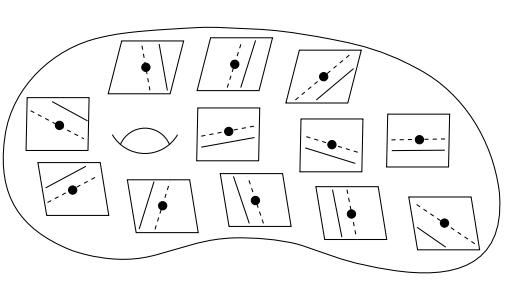
\includegraphics[scale = 0.45]{covector_fields.png}}
\end{minipage}
\caption{\scriptsize
\textbf{A covector field}}
\label{fig: covector_fields}
\end{figure}

\item \begin{remark}
Note that a nonzero linear functional $\omega_{p} \in T_{p}^{*}M$ is completely determined by two pieces of data: its \emph{\textbf{kernel}}, which is a linear hyperplane in $T_{p}M$ (\emph{a codimension-$1$ linear subspace}); and the set of vectors $v$ for which $\omega_p(v) = 1$, which is \emph{an \textbf{affine hyperplane parallel to the kernel}} (Fig. \ref{fig: covector_fields})  The value of $\omega_{p}(v)$ for any other vector $v$ is then obtained by linear interpolation or extrapolation.
\end{remark}

\item \begin{remark} (\textbf{\emph{Visualize the Vector Fields and the Covector Fields}})
\begin{enumerate}
\item A vector field on $M$ can be considered as an arrow attached to each point of $M$.
\item A covector field on $M$ can be considered as defining \emph{\textbf{a pair of hyperplanes}} in each tangent space, \emph{one \textbf{through the origin}} and \emph{another \textbf{parallel} to it}, and varying continuously from point to point. 

Where the covector field is small, one of the hyperplanes becomes \emph{very far from the kernel}, eventually disappearing altogether at points where the covector field takes the value zero.
\end{enumerate}
\end{remark}

\end{itemize}

\section{The Differential of a Function}
\begin{itemize}
%\item Note that for real-valued function $f: \bR^{n} \rightarrow \bR$,  the \emph{\textbf{gradient}} of $f$ is defined as the \emph{\textbf{vector field}} whose components are the partial derivatives of $f$. It can be written as  
%\begin{align*}
%\nabla f &= \sum_{i=1}^{n}\partdiff{f}{x^{i}}\partdiff{}{x^{i}}.
%\end{align*} Unfortunately, in this form, the gradient does not make sense independently of coordinates. 

\item \begin{remark}
Although \emph{\textbf{the partial derivatives of a smooth function}} cannot be interpreted in a \emph{coordinate-independent way} as the \emph{components} of \emph{a vector field}, it turns out that they \emph{can} be interpreted as the \emph{\textbf{components of a covector field}}. This is \emph{the most important application} of covector fields.
\end{remark}

\item  \begin{definition}
Let $f$ be a \emph{smooth real-valued function} on a \emph{smooth manifold} $M$ with or without boundary. (As usual, all of this discussion applies to functions defined on an open subset $U \subseteq M$; simply by \emph{replacing} $M$ with $U$ throughout.) We define a \emph{\textbf{covector field}} $df$ , called \underline{\emph{\textbf{the differential of $f$}}}, by
\begin{align*}
df_{p}(v) &= v\,f, \quad \forall v\in T_{p}M.
\end{align*}
\end{definition}

\item \begin{proposition}
The differential of a smooth function is a smooth covector field.
\end{proposition}

\item \begin{remark}
Similar to comparison between \emph{tangent vector} $v \in T_{p}M$ and \emph{tangent vector field} $X$, the \emph{differential of $f$} is a \emph{\textbf{covector field}}, i.e. a smooth function that maps a point $p$ to covector $df_{p}$, the differential of $f$ \emph{at $p$}. $df$ can be seen as a global concept that summarizes information of differential maps across the manifold. 
\end{remark}

\item \begin{remark} (\emph{\textbf{Coordinate Representation of differential of $f$}})\\
Let $(x^i)$ be smooth coordinates on an open subset $U \subseteq M$, and let $(\lambda^i)$ be the corresponding \emph{coordinate coframe} on $U$. Write $df$ in coordinates as $df_p = A_i(p) \lambda^i |_p$ for some functions $A_i: U \rightarrow \bR$,  then the definition of $df$ implies
\begin{align*}
A_i(p) &= df_{p}\paren{\partdiff{}{x^{i}}\Bigr|_{p}} = \partdiff{}{x^{i}}\Bigr|_{p} f = \partdiff{f}{x^{i}}(p).
\end{align*} This yields the following formula for \emph{\textbf{the coordinate representation of $df$}}:
\begin{align}
df_p = \partdiff{f}{x^{i}}(p) \; \lambda^i |_p \label{eqn: differential_coordinate_representation_0}
\end{align} Thus, the \emph{\textbf{component functions}} of $df$ in any smooth coordinate chart are \emph{\textbf{the partial derivatives of $f$} with respect to those coordinates}. Because of this, we can think of $df$ as \emph{an analogue of the classical gradient}, reinterpreted in a way that makes \emph{coordinate-independent sense} on a manifold.

If we apply \eqref{eqn: differential_coordinate_representation_0} to the special case in which $f$ is one of the \emph{coordinate functions} $x^j: U \rightarrow \bR$, we obtain
\begin{align*}
d x^{j} |_p  &= \partdiff{x^{j}}{x^{i}}(p) \; \lambda^i |_p = \delta_{i}^{j}\; \lambda^i |_p =  \lambda^j |_p.
\end{align*}

In other words, \emph{\textbf{the coordinate covector field $\lambda^j$} is none other than \textbf{the differential $dx^j$}}. Therefore, the formula \eqref{eqn: differential_coordinate_representation_0} for $df_p$ can be rewritten as
\begin{align}
df_p = \partdiff{f}{x^{i}}(p) \; d x^{i} |_p.   \label{eqn: differential_coordinate_representation_1}
\end{align} or as \emph{\textbf{an equation between covector fields}} instead of covectors. The \emph{\textbf{coordinate representation of differential $df$}} is
\begin{align}
df = \partdiff{f}{x^{i}} \; d x^{i}.   \label{eqn: differential_coordinate_representation}
\end{align} Thus, we have recovered the familiar classical expression for the differential of a
function $f$ in coordinates. Henceforth, we abandon the notation $\lambda^i$ for the coordinate coframe, and use $dx^i$ instead. 

The \underline{\emph{\textbf{coordinate representation of covector field $\omega$}}} is
\begin{align}
&\omega = \omega_i\, dx^i \label{eqn: covector_field_coordinate_representation} \\
&\text{where } dx^{i}\paren{\partdiff{}{x^{j}}\Bigr|_{p}} = \delta_{j}^{i}, \quad \forall i,j =1,\ldots, n, p \in M \nonumber
\end{align}

\end{remark}

\item \begin{remark} The equation \eqref{eqn: covector_field_coordinate_representation} should be considered as \emph{the \textbf{equation} between \textbf{covector field}} $df$ and \emph{the corresponding \textbf{coordinate covector fields}} $dx^{i}, i=1,\ldots, n$. This is derived without using the total differential equation from \emph{the multivariate calculus}. The linear cooefficients for the combination is \emph{the partial derivatives of $f$}.
\end{remark}

\begin{figure}[htb]
\centering
\begin{minipage}{0.5\linewidth}
 \centerline{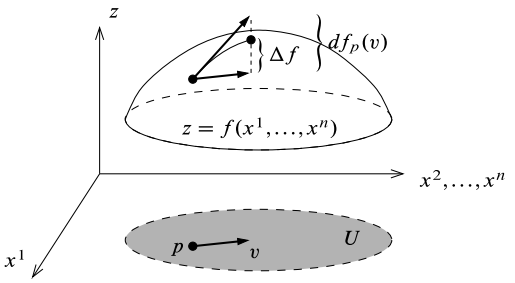
\includegraphics[scale = 0.5]{differential_as_rate_of_change.png}}
\end{minipage}
\caption{\scriptsize
\textbf{The differential $df$ can be seen as rate of changes of $f$ along curve $\gamma$}}
\label{fig: differential_as_rate_of_change}
\end{figure}

\item \begin{proposition} (\textbf{Properties of the Differential}).\\
Let $M$ be a smooth manifold with or without boundary, and let $f, g \in \cC^{\infty}(M)$.
\begin{enumerate}
\item If $a$ and $b$ are constants, then $d(a\,f + b\,g) = a\, df + b\, dg$.
\item $d (f\,g) = f\, dg + g\, df$.
\item $d (f / g) = (g\, df  - f\, dg) / g^2$ on the set where $g \neq 0$.
\item If $J \subseteq \bR$ is an interval containing the image of $f$, and $h: J \rightarrow \bR$ is a smooth function, then $d (h \circ f) = (h' \circ f) \,df$ .
\item If $f$ is constant, then $df = 0$.
\end{enumerate}
\end{proposition}

\item \emph{\textbf{One very important property}} of the differential is the following characterization of smooth functions with vanishing differentials.
\begin{proposition} (\textbf{Functions with Vanishing Differentials}). \citep{lee2003introduction} \\
If $f$ is a smooth real-valued function on a smooth manifold $M$ with or without boundary, then $df = 0$ if and only if $f$ is \textbf{constant} on \textbf{each component} of $M$ .
\end{proposition}


\item \begin{remark} Suppose $M$ is a smooth manifold and $f \in \cC^{\infty}(M)$, and let $p$ be a point in $M$. By choosing smooth coordinates on a neighborhood of $p$, we can think of $f$ as a function on an open subset $U\subseteq \bR^n$.  Recall that $dx^i |_p$ is the \emph{linear functional that picks out the $i$-th component of a tangent vector} at $p$.  Writing $\Delta f = f(p + v) - f(p)$ for $v\in \bR^{n}$, Taylor’s theorem shows that $f$ is well approximated when $v$ is small by
\begin{align*}
\Delta f = f(p + v) -  f(p)  &\approx \partdiff{f}{x^{i}}(p) v^{i} = \partdiff{f}{x^{i}}(p) dx^{i}(v) = df_{p} (v).
\end{align*} In other words, \emph{\textbf{$df_p$ is the linear functional that best approximates $f$ near $p$.}} (See Fig \ref{fig: differential_as_rate_of_change}).

The great power of the concept of the differential comes from the fact that we can define df \emph{\textbf{invariantly}} on any manifold, without resorting
to vague arguments involving \emph{infinitesimals}.
\end{remark}

\begin{figure}[tb]
\centering
\begin{minipage}{0.5\linewidth}
 \centerline{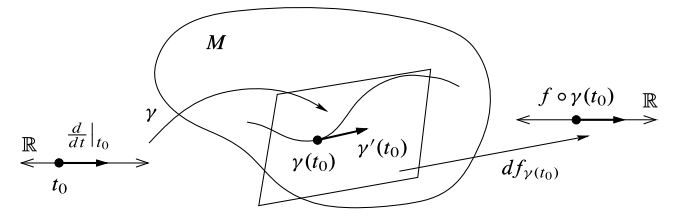
\includegraphics[scale = 0.5]{derivation_function_along_curve.png}}
\end{minipage}
\caption{\scriptsize
\textbf{The derivative of  $f$ along curve $\gamma$}}
\label{fig: derivation_function_along_curve}
\end{figure}

\item \begin{proposition}(\textbf{Derivative of a Function Along a Curve}). \\
Suppose $M$ is a smooth manifold with or without boundary, $\gamma:  J \rightarrow M$ is a smooth curve, and $f: M \rightarrow \bR$ is a smooth function. Then the \textbf{derivative} of the real-valued function $f \circ \gamma:  J \rightarrow \bR$ is given by
\begin{align}
(f \circ  \gamma)'(t) &=  df_{\gamma(t)}(\gamma'(t)). \label{eqn: differential_rate_of_change_curve}
\end{align}
\end{proposition}
\begin{proof} For any $t_0 \in J$
\begin{align*}
 df_{\gamma(t_0)}(\gamma'(t_0)) &= \gamma'(t_0) f \quad (\text{by definition of }df)\\
 &= d \gamma_{t_0}\paren{\frac{d}{dt}\Bigr|_{t_0}}f  \quad (\text{by definition of }\gamma')\\
 &=\frac{d}{dt}\Bigr|_{t_0} \paren{f \circ \gamma} \quad (\text{by definition of }d\gamma)\\
 &= (f \circ  \gamma)'(t_0). \qed
\end{align*}
\end{proof}



\item \begin{remark}
You may have noticed that for a smooth real-valued function $f: M \rightarrow \bR$, we now have \emph{\textbf{two different definitions}} for \emph{the differential of $f$} at a point $p \in M$. 
\begin{enumerate}
\item we defined $df_p$ as \emph{\textbf{a linear map}} from $T_{p}M$ to $T_{f(p)}\bR$, i.e. \emph{\textbf{a linear operator}} that maps a tangent vector in $T_pM$ to another tangent vector in $T_{f(p)}\bR$.
\item we defined $df_p$ as \emph{\textbf{a covector at $p$}}, which is to say a linear map from $T_{p}M$ to $\bR$, i.e. \emph{\textbf{a linear functional}} on $T_pM$.
\end{enumerate}
\end{remark}

\item \begin{remark}
Similarly, if $\gamma$ is a smooth curve in $M$, we have \textbf{\emph{two different meanings}} for the expression $(f \circ  \gamma)'(t)$:
 \begin{enumerate}
 \item $(f \circ \gamma)$ can be interpreted as a smooth curve in $\bR$, and thus $(f \circ  \gamma)'(t)$ is its \emph{\textbf{velocity}} at the point $f \circ  \gamma(t)$, which is an element of \emph{\textbf{the tangent space}}  $T_{f\circ\gamma(t)}\bR$.  By \eqref{eqn: differential_rate_of_change_curve}, we see that it equal to $df_{\gamma(t)}(\gamma'(t))$, as \emph{\textbf{a tangent vector}}.
 \item $(f \circ \gamma)$ can also be considered simply as a real-valued function of one real variable, and then $(f \circ  \gamma)'(t)$ is just its \emph{\textbf{ordinary derivative}}. By \eqref{eqn: differential_rate_of_change_curve}, we see that it equal to $df_{\gamma(t)}(\gamma'(t))$, \emph{\textbf{as a real number}}.
 \end{enumerate}
\end{remark}
\end{itemize}


\section{Pullbacks of Covector Fields}
\subsection{Definitions}
\begin{itemize}
\item Recall that for diffeomorphism $F: M\rightarrow N$, the \emph{\textbf{pushforward of a vector field $X$ by $F$}}, denoted as $F_{*}X$ or $F_{\#}X$ is \emph{the unique vector field} obtained by differential of $F$ acting on $X$.  
\begin{align*}
(F_{*}X)_{q} &= dF_{F^{-1}(q)}\paren{X_{F^{-1}(q)}}, \quad q \in N.
\end{align*}

\emph{Dualizing} this process leads to a linear map on covectors going \emph{in the opposite direction}.

\item \begin{definition}
Let $F: M \rightarrow N$ be a \emph{smooth map} between smooth manifolds with or without boundary, and let $p \in M$ be arbitrary. The differential $dF_p: T_{p}M \rightarrow T_{F(p)}N$ yields \emph{a \textbf{dual linear map}}
\begin{align*}
dF_{p}^{*}:  T_{F(p)}^{*}N \rightarrow T_{p}^{*}M,
\end{align*} called \underline{\emph{\textbf{the (pointwise) pullback by $F$ at $p$}}, or \textbf{\emph{the cotangent map} of $F$}}. Unraveling
the definitions, we see that $dF_{p}^{*}$ is characterized by
\begin{align*}
dF_{p}^{*}(\omega)(v) &= \omega(dF_{p}(v)), \quad  \omega \in T_{F(p)}^{*}N, \; v \in T_{p}^{*}M.
\end{align*}
\end{definition}

\item \begin{definition}
Given a smooth map $F: M \rightarrow N$ and a \emph{covector field} $\omega$ on $N$ , define a \emph{\textbf{rough covector field}} $F^{*}\omega$ on $M$, called the
\textbf{\emph{pullback of $\omega$ by $F$}}, by
\begin{align*}
(F^{*}\omega)_p &= dF_{p}^{*}\paren{\omega_{F(p)}}
\end{align*}  We also denote \emph{the pullback of $\omega$ by $F$as $F^{\#}\omega$}.
\end{definition}

\item \begin{remark}
Observe that the assignments $(M, p)\mapsto T_{p}^{*}M$ and $F \mapsto dF_{p}^{*}$ yield a \emph{contravariant functor} from the category of pointed smooth manifolds to the category of real vector spaces. 
\end{remark}

\item \begin{remark}
Although the \emph{pushforward of a vector field by $F$}, $F_{\#}X$, is only uniquely defined for \emph{diffeomorphism} $F$, the \emph{pullback of a covector field by $F$}, $F^{\#}\omega$, is \textbf{\emph{always unique}}.    

It acts on a vector $v \in T_{p}M$ by
\begin{align*}
(F^{\#}\omega)_{p}(v) = dF^{\#}_{p}(\omega_{F(p)})(v) = \omega_{F(p)}(dF_{p}(v)) 
\end{align*}
\end{remark}


\item \begin{proposition} Let $F: M \rightarrow N$ be a smooth map between smooth manifolds with or without boundary. Suppose $u$ is a \emph{continuous real-valued} function on $N$, and $\omega$ is a covector field on $N$. Then
\begin{align}
F^{*}(u\, \omega) &= (u \circ F) F^{*}\omega \label{eqn: pullback_product_rule}
\end{align} If in addition $u$ is smooth, then
\begin{align}
F^{*}du  &=  d(u \circ F) \label{eqn: pullback_composite_rule}
\end{align}
\end{proposition}
\begin{proof}
To proof \eqref{eqn: pullback_product_rule}, we compute:
\begin{align*}
(F^{*}(u\, \omega))_{p} &= dF_{p}^{*}((u \, \omega)_{F(p)}) \quad (\text{by definition of pullback of covector field})\\
&= dF_{p}^{*}(u(F(p)) \, \omega_{F(p)}) \quad (\text{by smooth function times vector field })\\
&= u(F(p)) \, dF_{p}^{*}(\omega_{F(p)}) \\
&= (u \circ F)(p)\, (F^{*}\omega)_{p} = \paren{ (u \circ F) F^{*}\omega}_{p}
\end{align*}
To proof \eqref{eqn: pullback_composite_rule}, we compute for every $p \in M, v\in T_{p}M$
\begin{align*}
(F^{*}du)_{p}(v) &=  dF_{p}^{*}(du_{F(p)})(v) \quad (\text{by definition of pullback of covector field})\\
&= du_{F(p)}\paren{dF_{p}(v)} \quad (\text{by definition of pullback of covector at $p$})\\
&= dF_{p}(v) u \quad (\text{by definition of $du$})\\
&= v(u \circ F) \quad (\text{by definition of $dF_{p}$})\\
&= d(u \circ F)_{p}(v) \quad (\text{by definition of $d(u \circ F)$})
\end{align*}
\qed
\end{proof}

\item \begin{proposition}
Suppose $F: M \rightarrow N$  is a smooth map between smooth manifolds with or without boundary, and let $\omega$ be a covector field on $N$. Then $F^{*}\omega$ is a
\textbf{(continuous) covector field} on $M$. If $\omega$ is smooth, then so is $F^{*}\omega$.
\end{proposition}

\item \begin{remark} (\emph{\textbf{Coordinate Representation of Pullback Covector Fields}})\\
Given the  coordinate representation of covector  $\omega = \omega_{j}dy^{j}$, the pullback of a covector field  can also be written in the
following way:
\begin{align}
F^{*}\omega &= F^{*}(\omega_{j}dy^{j}) \nonumber\\
&= (\omega_{j} \circ F) F^{*}(dy^{j}) \nonumber\\
&= (\omega_{j} \circ F)\, d\paren{y^{j} \circ F}  \label{eqn: pullback_covector_field_decompo_1}\\
&= (\omega_{j} \circ F) \,d\,F^{j}  \label{eqn: pullback_covector_field_decompo_2}
\end{align} where  $F^j$ is the $j$ th component function of $F$ in these coordinates. Using either of
these formulas, the computation of pullbacks in coordinates is exceedingly simple.

In other words, to compute $F^{*}\omega$, all you need to do is \emph{\underline{\textbf{substitute}} the \textbf{component functions} of $F$ for the \underline{\textbf{coordinate functions} of $N$} everywhere they appear in $\omega$}.
\end{remark}

\item \begin{remark} Get familiar with the following expressions:
\begin{enumerate}
\item For $g \in \cC^{\infty}(N)$, $q = F(p) \in N$ so that $p= F^{-1}(q) \in M$, 
\begin{align*}
(F_{*}X)_{q}\,g &= dF_{p}(X_{p})g = X_{p}\paren{g \circ F} 
\end{align*}

\item For $p\in M$, $X_{p} \in T_{p}M$, $q = F(p) \in N$, $\omega_{q} \in T_{q}^{*}N$, 
\begin{align*}
(F^{*}\omega)_{p}(X_{p}) &= \paren{dF_{p}^{*}\omega_{q}}\paren{X_{p}} = \omega_{q}\paren{dF_{p}(X_{p})}
\end{align*} The last equality use the definition of dual map $(A^{*}w)(v) = w(A\,v)$

\item For a diffeomorphism $F$, $(F^{*})^{-1} = F_{*}$. That is \textbf{\emph{the inverse of pullback operation is the pushforward operation}}.
\end{enumerate}
\end{remark}
\end{itemize}


\subsection{Restricting Covector Fields to Submanifolds}
\begin{itemize}
\item \begin{remark}
Compare to restricting vector fields to submanifolds, the restriction of covector fields to submanifolds is much simpler.
\end{remark}

\item \begin{remark} (\emph{\textbf{The Pullback of Covector Field by the Inclusion Map is a Covector Field on Submanifold}})\\
Suppose $M$ is a smooth manifold with or without boundary, $S \subseteq M$ is an \emph{\textbf{immersed submanifold}} with or without boundary, and $\iota: S \xhookrightarrow{} M$ is \emph{the inclusion map}. If $\omega$ is any smooth covector field on $M$, \emph{\textbf{the pullback by $\iota$ yields a smooth covector
field $\iota^{*}\omega$ on $S$}}. 

To see what this means, let $v \in T_{p}S$ be arbitrary, and compute
\begin{align*}
(\iota^{*}\omega)_p(v) = \omega_p\paren{d\iota_p(v)} = \omega_p(v).
\end{align*} since $d\iota_p: T_{p}S \rightarrow T_{p}M$ is just the inclusion map, under our usual identification of $T_{p}S$ with a subspace of $T_{p}M$. Thus, $\iota^{*}\omega$ is just the restriction of $\omega$ to vectors tangent to $S$. For this reason, $\iota^{*}\omega$ is often called \underline{\emph{\textbf{the restriction of $\omega$ to $S$}}}. 

Be warned, however, that $\iota^{*}\omega$ might equal \textbf{\emph{zero}} at a given point of $S$, even though \emph{\textbf{considered as a covector field on $M$}}, \emph{\textbf{$\omega$ might not vanish there}}. 
\end{remark}

\item \begin{example} ($\omega \neq 0$ but $\iota^{*}\omega = 0$)\\
Let $\omega = dy$ on $\bR^2$, and let $S$ be the $x$-axis, considered as an embedded submanifold of $\bR^2$. As a covector field on $\bR^2$, $\omega$ is \textbf{\emph{nonzero}} everywhere, because one of its component functions is \emph{\textbf{always} $1$}. However, the restriction $\iota^{*}\omega$ is
\emph{\textbf{identically zero}}, because $y$ vanishes identically on $S$:
\begin{align*}
\iota^{*}\omega = \iota^{*} dy = d(y \circ \iota) = 0.
\end{align*}
\end{example}

\item \begin{remark}
One usually says that ``\emph{\textbf{$\omega$ vanishes along $S$}}" or ``\emph{\textbf{$\omega$ vanishes at points of $S$}}"
if $\omega_p = 0$ for every point $p \in S$. 

The \emph{\textbf{weaker condition}} that $\iota^{*}\omega = 0$ is expressed by saying that ``\emph{\textbf{\underline{the restriction of} $\omega$ to $S$ vanishes}}", or ``\emph{\textbf{\underline{the pullback of $\omega$} to $S$ vanishes}}".
\end{remark}

\end{itemize}

\newpage

\section{Compare Tangent Bundle and Cotangent Bundle}
\begin{table}[h!]
\setlength{\abovedisplayskip}{0pt}
\setlength{\belowdisplayskip}{-10pt}
\setlength{\abovedisplayshortskip}{0pt}
\setlength{\belowdisplayshortskip}{0pt}
\centering
\caption{Comparison between tangent space and cotangent space}
\label{tab: tangent_cotangent}
%\setlength{\extrarowheight}{1pt}
\renewcommand\tabularxcolumn[1]{m{#1}}
\footnotesize
\begin{tabularx}{1\textwidth} { 
  | >{\raggedright\arraybackslash} m{2cm}
  | >{\centering\arraybackslash}X
  | >{\centering\arraybackslash}X  | }
 \hline
 base &  \emph{\textbf{smooth manifold}} $M$ & \emph{\textbf{smooth manifold}} $M$  \\
 \hline
 element  & $\varphi(p) = (x^1, \ldots, x^{n})$ & $\varphi(p) = (x^1, \ldots, x^{n})$\\
\hline
vector space (\emph{\textbf{fiber}}) at $p$ &  \textbf{tangent space}  $T_{p}M$ &  \textbf{cotangent space} $T_{p}^{*}M = (T_{p}M)^{*}$ \\
\hline
dimension of vector space & $n$ & $n$  \\
\hline
basis of vector space & 
\vspace{-1.25em}
\begin{align*}
 \paren{\dfrac{\partial}{\partial x^{1}}\Bigr|_{p}, \ldots, \dfrac{\partial}{\partial x^{n}}\Bigr|_{p}}
\end{align*}
\vspace{-1em}
 &   
\vspace{-1.25em}
\begin{align*}
 (dx^1\bigr|_{p}, \ldots, dx^n\bigr|_{p})
\end{align*} \vspace{-1em}\\
\hline
element in vector space   &
\vspace{-1.25em}
 \begin{align*} 
\text{\textbf{tangent vector} }:\cC^{\infty}(M) \rightarrow \bR\\
  v = v^{i}\dfrac{\partial}{\partial x^{i}}\Bigr|_{p}
 \end{align*} \vspace{-1em}  & 
\vspace{-1.25em} 
 \begin{align*} 
 \text{\textbf{cotangent vector} }:T_pM \rightarrow \bR\\
 \omega = \xi_{i}\;dx^i\bigr|_{p}
 \end{align*} \vspace{-1em} \\
\hline
total space of \emph{\textbf{bundle}}   & 
\vspace{-1.25em}
\begin{align*}
 \text{\textbf{tangent bundle} }\\
TM =  \bigsqcup_{p\in M}T_{p}M
 \end{align*} 
 & 
 \vspace{-1.25em}
\begin{align*}
 \text{\textbf{cotangent bundle} }\\
T^{*}M =  \bigsqcup_{p\in M}T_{p}^{*}M, 
 \end{align*}\\
\hline
element in bundle &
$(x^1(p), \ldots, x^{n}(p),  v^1, \ldots, v^{n})$
& 
$(x^1(p), \ldots, x^{n}(p),  \xi_1, \ldots, \xi_{n})$ \\
\hline
\emph{\textbf{section}}  &  
\vspace{-1.25em}
\begin{align*}
\text{\textbf{local vector field} }\\
X = X^{i}\partdiff{}{x^{i}}\\
X_{p} \in T_{p}M
\end{align*} \vspace{-1.25em}
&
\vspace{-1.25em}
\begin{align*}
\text{\textbf{local covector field} }\\
\omega = \xi_{i} dx^{i}\\
\omega_p \in T_{p}^{*}M
\end{align*} \vspace{-1.25em} \\
\hline
vector space of sections & $\mathfrak{X}(M) \equiv \Gamma(TM)$ & $\mathfrak{X}^{*}(M) \equiv \Gamma(T^{*}M)$ \\
\hline
\emph{\textbf{frame}} 
&
\vspace{-1.25em}
\begin{align*}
\text{\textbf{coordinate vector fields}}\\
\paren{\partdiff{}{x^{1}}, \ldots, \partdiff{}{x^{n}}}
\end{align*} \vspace{-1em} &
\vspace{-1.25em}
\begin{align*}
\text{\textbf{coordinate covector fields}}\\
\paren{dx^1, \ldots, dx^{n}}
\end{align*} \vspace{-1em}\\
\hline
\emph{\textbf{duality}} & 
\vspace{-1.25em}
\begin{align*}
\xi\paren{\partdiff{}{x^{i}}\Bigr|_{p}}(dx^{j}|_{p}) = \delta_{i}^{j}
\end{align*} \vspace{-1em} &
\vspace{-1.25em}
\begin{align*}
dx^{j}|_{p}\paren{\partdiff{}{x^{i}}\Bigr|_{p}} = \delta_{i}^{j}
\end{align*} \vspace{-1em} \\
\hline
\emph{\textbf{change of coordinates}} &
\vspace{-1.25em}
\begin{align*}
\text{\textbf{contravariant}}\\
\widetilde{v}^{j}= \partdiff{\widetilde{x}^{j}}{x^{i}}(p)\, v^{i}
\end{align*}\vspace{-1em}
&
\vspace{-1.25em}
\begin{align*}
\text{\textbf{covariant}}\\
\omega_{i} = \partdiff{\widetilde{x}^{j}}{x^{i}}(p)\,\widetilde{\omega}_{j}
\end{align*}\vspace{-1em}
\\
\hline
\emph{\textbf{functions}} &
\vspace{-1.25em}
\begin{align*}
F: M \rightarrow N\text{ \emph{\textbf{diffeomorphism}}}\\
dF_{p}: T_pM \rightarrow T_{F(p)}N \\
\text{\emph{\textbf{Pushforward}}: }F_{*}: \mathfrak{X}(M) \rightarrow \mathfrak{X}(N)  \\
(F_{*}X)_{q} = dF_{F^{-1}(q)}(X_{F^{-1}(q)}),\; q\in N
\end{align*}\vspace{-1em}
&
\vspace{-1.25em}
\begin{align*}
\\
dF_{p}^{*}:  T_{F(p)}^{*}N \rightarrow T_{p}^{*}M \text{ \emph{\textbf{dual map of }}}dF_p\\
\text{\emph{\textbf{Pullback}}: }F^{*}: \mathfrak{X}^{*}(N) \rightarrow \mathfrak{X}^{*}(M)\\
(F^{*}\omega)_p = dF_{p}^{*}\paren{\omega_{F(p)}},\; p\in M
\end{align*} \vspace{-1em}
\\
\hline
\end{tabularx}
\end{table}


\section{Line Integrals}

\section{Conservative Covector Fields}
\begin{itemize}
\item \begin{definition}
A \emph{smooth covector field} $\omega$ on a smooth manifold $M$ with or without boundary is said to be \underline{\emph{\textbf{exact}}} (or \emph{an \textbf{exact differential}}) on $M$ if there is a function $f \in \cC^{\infty}(M)$ such that $\omega = df$. In this case, the function $f$ is called \underline{\emph{\textbf{a potential} for $\omega$}}.
\end{definition}

\item \begin{definition}
A curve $\gamma: [a,b]\rightarrow M$ is a \emph{\textbf{closed curve segment}} if $\gamma(a) = \gamma(b)$. The integral of $df$ over $\gamma$ is \emph{\textbf{zero}}.
\end{definition}

\item \begin{definition}
A smooth covector field $\omega$ is said to be \underline{\emph{\textbf{conservative}}} if the line integral of $\omega$ over \emph{every piecewise smooth \textbf{closed} curve segment} is \emph{\textbf{zero}}. 
\end{definition}

\item \begin{proposition}
A smooth covector field $\omega$ is conservative if and only if its line integrals are \textbf{path-independent}, in the sense that $\int_{\gamma}\omega = \int_{\widetilde{\gamma}}\omega$ whenever $\gamma$ and $\widetilde{\gamma}$ are piecewise smooth curve segments with the \textbf{same} starting and ending points.
\end{proposition}

\item \begin{theorem}
Let $M$ be a smooth manifold with or without boundary. A smooth covector field on $M$ is \textbf{conservative} if and only if it is \textbf{exact}.
\end{theorem}

\item \begin{remark}
To check whether a given covector field is exact, there is a very simple \emph{\textbf{necessary condition}}, which follows from the fact that \emph{\textbf{partial derivatives} of smooth functions can be taken in \textbf{any order}}.
\end{remark}

\item \begin{remark}
Suppose $\omega \in \frX^{*}(M)$ is \textbf{\emph{exact}}. Let $f$ be any potential function for $\omega$, and let $(U, (x^i))$ be any smooth chart on $M$. Because $f$ is
smooth, it satisfies the following identity on $U$:
\begin{align}
\partdiff{f}{x^{i}\partial x^{j}} = \partdiff{f}{x^{j}\partial x^i} \label{eqn: exact_covector_field_2nd_order_partial_derivative}
\end{align}
Writing $\omega = \omega_i dx^{i}$ in coordinates, we see that $\omega = df$ is equivalent to $\omega_i =
\partial f / \partial x^i$. Substituting this into \eqref{eqn: exact_covector_field_2nd_order_partial_derivative}, we find that the component functions of $\omega$
satisfy the following identity \emph{for \textbf{each pair} of indices $i$ and $j$}:
\begin{align}
 \partdiff{\omega_{j}}{x^{i}}= \partdiff{\omega_i}{x^{j}}. \label{eqn: exact_covector_field_omega_partial_derivative}
\end{align} We say that \underline{a \emph{smooth covector field} $\omega$ is \emph{\textbf{closed}}} if its components in every smooth
chart satisfy \eqref{eqn: exact_covector_field_omega_partial_derivative}. The following proposition summarizes the computation above.

\begin{proposition}
Every exact covector field is closed.
\end{proposition}
\end{remark}

\item \begin{proposition}
Let $\omega$ be a smooth covector field on a smooth manifold $M$ with or without boundary. The following are equivalent:
\begin{enumerate}
\item $\omega$ is \textbf{closed}.
\item $\omega$ satisfies \eqref{eqn: exact_covector_field_omega_partial_derivative} in \textbf{some smooth chart} around \textbf{every point}.
\item For any open subset $U \subseteq M$ and smooth vector fields $X, Y \in \frX(U)$,
\begin{align}
X\paren{\omega\paren{Y}} - Y\paren{\omega\paren{X}} = \omega\paren{[X, Y]}.\label{eqn: exact_covector_field_vector_field_lie_bracket}
\end{align}
\end{enumerate}
\end{proposition}

\item \begin{corollary}
Suppose $F: M \rightarrow N$ is a \textbf{local diffeomorphism}. Then the \textbf{pullback} $F^{*}: \frX^{*}(N)  \rightarrow \frX^{*}(M)$ takes \textbf{closed} covector fields to \textbf{closed} covector fields, and \textbf{exact} ones to \textbf{exact} ones.
\end{corollary}
\end{itemize}


\newpage
\bibliographystyle{plainnat}
\bibliography{book_reference.bib}
\end{document}